\documentclass[12pt]{article}


% defining image path
\usepackage{graphicx}
\graphicspath{ {./images/} }

% tables
\usepackage[utf8]{inputenc}
\usepackage[table]{xcolor}
\usepackage{enumitem}
\usepackage{multirow}
% \usepackage{multicol}
% \usepackage{adjustbox}
% \usepackage{tabularx}
% \newcolumntype{L}{>{\raggedright\arraybackslash}X}
\setlist{nolistsep}

% rotate page
\usepackage{pdflscape}

\pagestyle{empty}
\setcounter{secnumdepth}{2}


\topmargin=0cm
\oddsidemargin=0cm
\textheight=22.0cm
\textwidth=16cm 

\parindent=0cm
\parskip=0.15cm
\topskip=0truecm
\raggedbottom
\abovedisplayskip=3mm
\belowdisplayskip=3mm
\abovedisplayshortskip=0mm
\belowdisplayshortskip=2mm
\normalbaselineskip=12pt
\normalbaselines

\begin{document}
\vspace*{0.5in}
\centerline{\bf\Large
Requirements for the Kakuro project}


\vspace*{0.5in}
\centerline{\bf\Large Iteration 2 COMP354}

\vspace*{0.5in}
\centerline{\bf\Large Team PK-A}

\vspace*{0.5in}
\centerline{\bf\Large 15 March 2020}

\vspace*{1.5in}
\begin{table}[htbp]
\caption{Team Members}
\begin{center}
\begin{tabular}{|c |c | c|}
\hline
Name & Role & ID Number \\
\hline\hline
Tiffany Ah King & Quality Control & 40082976 \\
\hline
Isabelle Charette & Documenter & 40008121 \\
\hline
Brian Gamboc-Javiniar & Coder & 40033124 \\
\hline
Vsevolod Ivanov & Organizer & 40004286 \\
\hline
Chang Liu & Quality Control & 40056360 \\
\hline
Nolan Mckay & Coder & 27873557 \\
\hline
Nalveer Moocheet & Quality Control & 40072605 \\
\hline
Hoang Thuan Pham & Coder & 40022992 \\
\hline
Audrey-Laure St-Louis & Documenter & 27558783 \\
\hline
Jia Ming Wei & Documenter & 40078192 \\
\hline
\end{tabular}
\end{center}
\end{table}


\newpage

\renewcommand*\contentsname{Table of Contents}

\tableofcontents

\clearpage

\section{Introduction}
\subsubsection{Introduction}
As a team, our goal is to develop the online Kakuro game. Through each iteration, we have been implementing uses cases, UI components and refactoring the structure of the code. By iteration 3, our goal is to have every component of the current online game implemented in our rendering of the game. 
\subsubsection{Purpose}
With this document, we will be presenting the design of the Kakuro game for the course COMP 354. In the following pages, we first explain in depth our choice of the Model View Controller (MVC) for the architectural design and implied subsystems. Next, we present the modules of the entailed detailed design of the MVC. Finally, we list dynamic scenarios which will describe the interaction between subsystems and units through execution scenarios.

\subsubsection{Scope}
In order to provide detailed design specifications of the Kakuro game and proceed efficiently with the development of the game, we present this documentation. The detailed explanations, definitions, UML diagrams and sequence diagrams provide the support needed for coherent implementation and communication between each role of the team. The documentation serves as a basis for depicting the software architecture of the game and understanding the implementation of the modules in the detailed design. The scope of this document is it to provide such support, which enables iteration 3 of our project for the Kakuro game.

\newpage

\section{Architectural Design} \label{sec:arch}




\begin{figure}[htbp]
    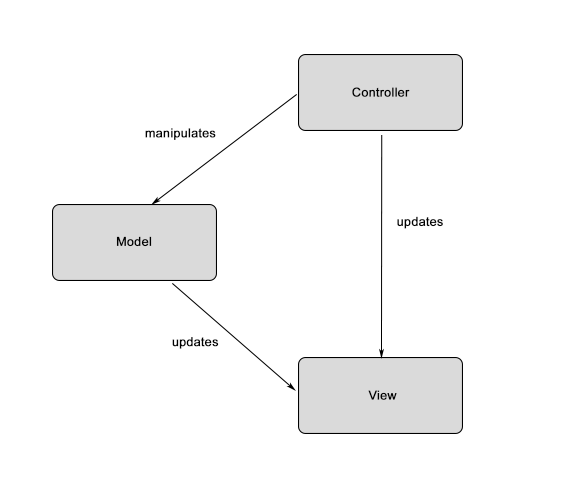
\includegraphics[width=0.7\textwidth]{MVC_part2}
    \caption{Architecture Diagram}
    \label{fig:archi_diagram}
\end{figure}

\subsection{Rationale}

The architecture chosen for the Kakuro game is the Model View Controller model (MVC). The MVC architecture is constructed of three separate components: the model, the view and the controller. \newline

The model is the central component of the game. It stores the data and it changes depending on the state of the game. In Kakuro, the model stores the information of the cells from the rows and the columns displayed by the graphical user interface. \newline

The view is the graphical user interface (GUI) of the game. It displays the grid, the buttons, and the text elements but it also displays the date from the model. It allows the player to enter numbers to play the game. Whenever the model changes, the GUI reacts to these changes by updating itself. \newline

The controller manages the interactions with the user and decides which functions should be called given an action. The controller will use the model’s data, he will take action on those depending on the user’s action and he will send it to the view for it to show it in the GUI.\newline




\subsection{Subsystem Interface Specifications}

\subsubsection{2.2.1 View Interface}

2.2.1.1 GameView \newline

The GameView class is the interface used for the View. With its constructor, it initializes the GUI of our Kakuro game. The following methods are available for this interface:
\newline
\begin{itemize}
\item getBoardUI (Cell) : Creates grid of cells by passing a 2D array of cells. Populates it properly and creates the GUI for it.
\item getMaxNumberValid() : Returns the maximum number valid for the player to use. In this game, the maximum value is 9
\item getMinNumberValid(): Returns the minimum number valid for the player to use. In this game, the minimum value is 1
\item getSavedInput() : Returns the UI component that are the cells of the boardgame
\item hideBoard(): Makes the current board not visible to the player
\item settingTextField(JTextField) : Sets the text field with colors and borders
\item showBoard() : Makes the current board visible to the player
\item updateView(): Removes a panel if one is already attached to the frame and save a reference to the new panel\newline
\end{itemize} 


2.2.1.2 MenuBarView\newline

The MenuBarView class is used for the different buttons displayed on the GUI of the game. The MenuBarView class contains the following methods:
\newline
\begin{itemize}
\item buttonsSetUp(): Sets up all the buttons (pause, resume, etc) by attaching an action listener to it
\item getMainPannel() : Returns the main panel of the game
\item toggleMenu(): Changes the state of the game by hiding the load and choose game buttons and setting visible all the other buttons (save, pause, resume, etc.) \newline
\end{itemize}

2.2.1.3 ChronoView\newline

The ChronoView class handles the chronometer of the game. It contains the following methods:\newline
\begin{itemize}
\item getTimerLabel() : Returns the timer label associated to the chronometer
\item setTimerLabel(String) : Sets the timer label given a string\newline
\end{itemize}


\subsubsection{2.2.2 Model Interface}
The interface between the controller and model is called whenever the controller receives input from the player. The kakuro.models package contains all the classes from the model interface. The following methods are part of the interface:\newline

2.2.2.1 GameModel \newline

The GameModel class is the interface used for the Model of our system. It interacts with the database and it generates the board game given the rules of the game. It contains the following methods:\newline
\begin{itemize}
\item getColumns() : Returns an integer value of the number of rows in the game
\item getRows() : Returns an integer value of the number of rows in the game
\item initBoard(): Creates the board game with the desired number of rows and columns and leave the cells empty\newline
\end{itemize}

2.2.2.2 ChronoModel\newline

The ChronoModel class is the model of the chronometer of our Kakuro game. It contains the following methods:\newline
\begin{itemize}
\item getDelay() : Returns the delay used for the chronometer
\item getHours() : Returns the hours value of the chronometer
\item getMinutes(): Returns the minutes value of the chronometer
\item getSeconds() Returns the seconds value of the chronometer
\item resetTimer() : Brings the chronometer to the value zero for its seconds, minutes and hours
\item setHours() : Sets the hours of the chronometer
\item setMinutes() : Sets the minutes of the chronometer
\item setSeconds() : Sets the seconds of the chronometer
\item updateTime(): Returns a string of the time given the increments of seconds, minutes and hours\newline
\end{itemize}

2.2.2.3 PlayerModel\newline

The PlayerModel class handles the player’s information. It contains the following methods:\newline
\begin{itemize}
\item getPlayerPassword() : Returns the password of the player
\item getPlayerUsername() : Returns the username of the player
\item setPlayerPassowrd() : Sets the password of the player
\item setPlayerUsername(): Sets the username of the player\newline
\end{itemize}





\subsubsection{2.2.3 Controller Interface}

The controller interface is a package (kakuro.controllers) composed of the following three classes:\newline

2.2.3.1 GameController\newline
The controller accepts input from the player and performs simple validations on it. The class contains the following methods : \newline
\begin{itemize}
\item connectDatabase() : Connects the game to the database
\item disconnectDatabase() : Disconnect the database from the game
\item getDatabaseConnection() : Returns the connections established from the database.
\item getMaxNumberValid() : Returns the maximum number aloud for the player to use during the game
\item getMinNumberValid() : Returns the minimum value aloud for the player to use during the game
\item getNumberFormatterClassType()
\item initGame(GameModel) : Given a GameModel, it initiate the game by initiating the board and it creates a chronoController and a menubarController
\item loadGame(): Upload the loaded game progress and display it in the GUI if it's available
\item loadInputInModel(): For every cells of every columns and rows, it loads it in the model when they are filled by the player
\item loadPreconfigureGame(int)
\item pause() : Pause the game which stops the chronometer and blocks the player from entering data in the game
\item restart() : Clears the board and restart the chronometer
\item resume() : Starts the chronometer and allows the player to continue playing by entering value in the board game
\item saveGame() : Save the state of the game in the database
\item solveBoard() : Solves the board by calculating the sums of the rows and the columns and checks if it brings to a correct solution. If the solution is correct, it returns true. Else it returns false
\item submit() : Lets the user get feedback from the system to know if he got the right solution or not \newline
\end{itemize}


2.2.3.2 MenuBarController\newline
\newline The MenuBarController Class accepts input from the player through the menu bar and performs actions depending on the button that is being pressed. The class contains the following methods:\newline
\begin{itemize}
\item getButtonMenuView() : Returns the buttonMenuView
\item getView() : Returns the main panel
\item isPaused() : Returns true if the game is paused. Else, it returns false
\item load() : Loads the game in the GUI
\item loadPreconfigureGame(GameDifficulty g): Given a game difficulty, loads it accordingly
\item pause(): Pauses the game
\item resume() : Resumes the game
\item save() : Saves the game in the database
\item submit() : Sends the current game for validation\newline
\end{itemize}



2.2.3.3 ChronoController\newline

The ChronoController class handles the actions that can be perform by the player and by the system itself on the chronometer. It contains the following methods: \newline
\begin{itemize}
\item chronoPause() : Pause the chronometer
\item chronoStart() : Starts the chronometer
\item getHours() : Returns the hours of the chronometer
\item getMinutes() : Returns the minutes of the chronometer
\item getSeconds() : Returns the seconds of the chronometer
\item getView():  Returns the label of the chronometer.
\item hide() : Hides the chronometer on the GUI of the game.
\item resetTimer() : Resets the chronometer to bring it to zero (hours, minutes and seconds)
show() : Display the chronometer in the GUI of the game
\item timerSetUp() : Set up the chronometer by attaching an action listener to it.
\item toggleTimerDisplay() : Sets the chronometer visible or hides it dependanding on the state he’s in\newline
\end{itemize}


\newpage

\section{Detailed Design} \label{sec:detail}

The Karuro system consists of three subsystems: the View module, the Model module, and the Controller module. This MVC model has been designed and implemented since the iteration 1. During the iteration 2, a SQLite server is integrated in the libraries so that the input data and solution data are possible to be stored in the database. The database is included in the Model module. The Controller module works like a router, routing the data flows between the Model module and the View module.  

\begin{figure}[htbp]
    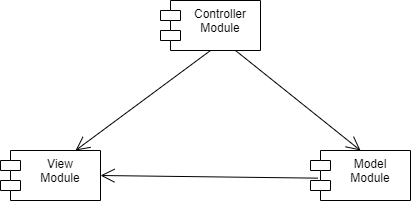
\includegraphics[width=1\textwidth]{Subsystems_UML}
    \caption{UML of Kakuro Subsystems}
    \label{fig:Subsystems_UML}
\end{figure}

The three subsystem or modules composite into one integrated system, the Karuro system. On the other hand, the three subsystems are independent of each other and interact with each other view their respective interfaces. This design practices the principles of high cohesion and low coupling. In this section the detailed design of the three modules will be described separately. Figure.3 shows all classes in the whole Kakuro system.


\begin{figure}[htbp]
    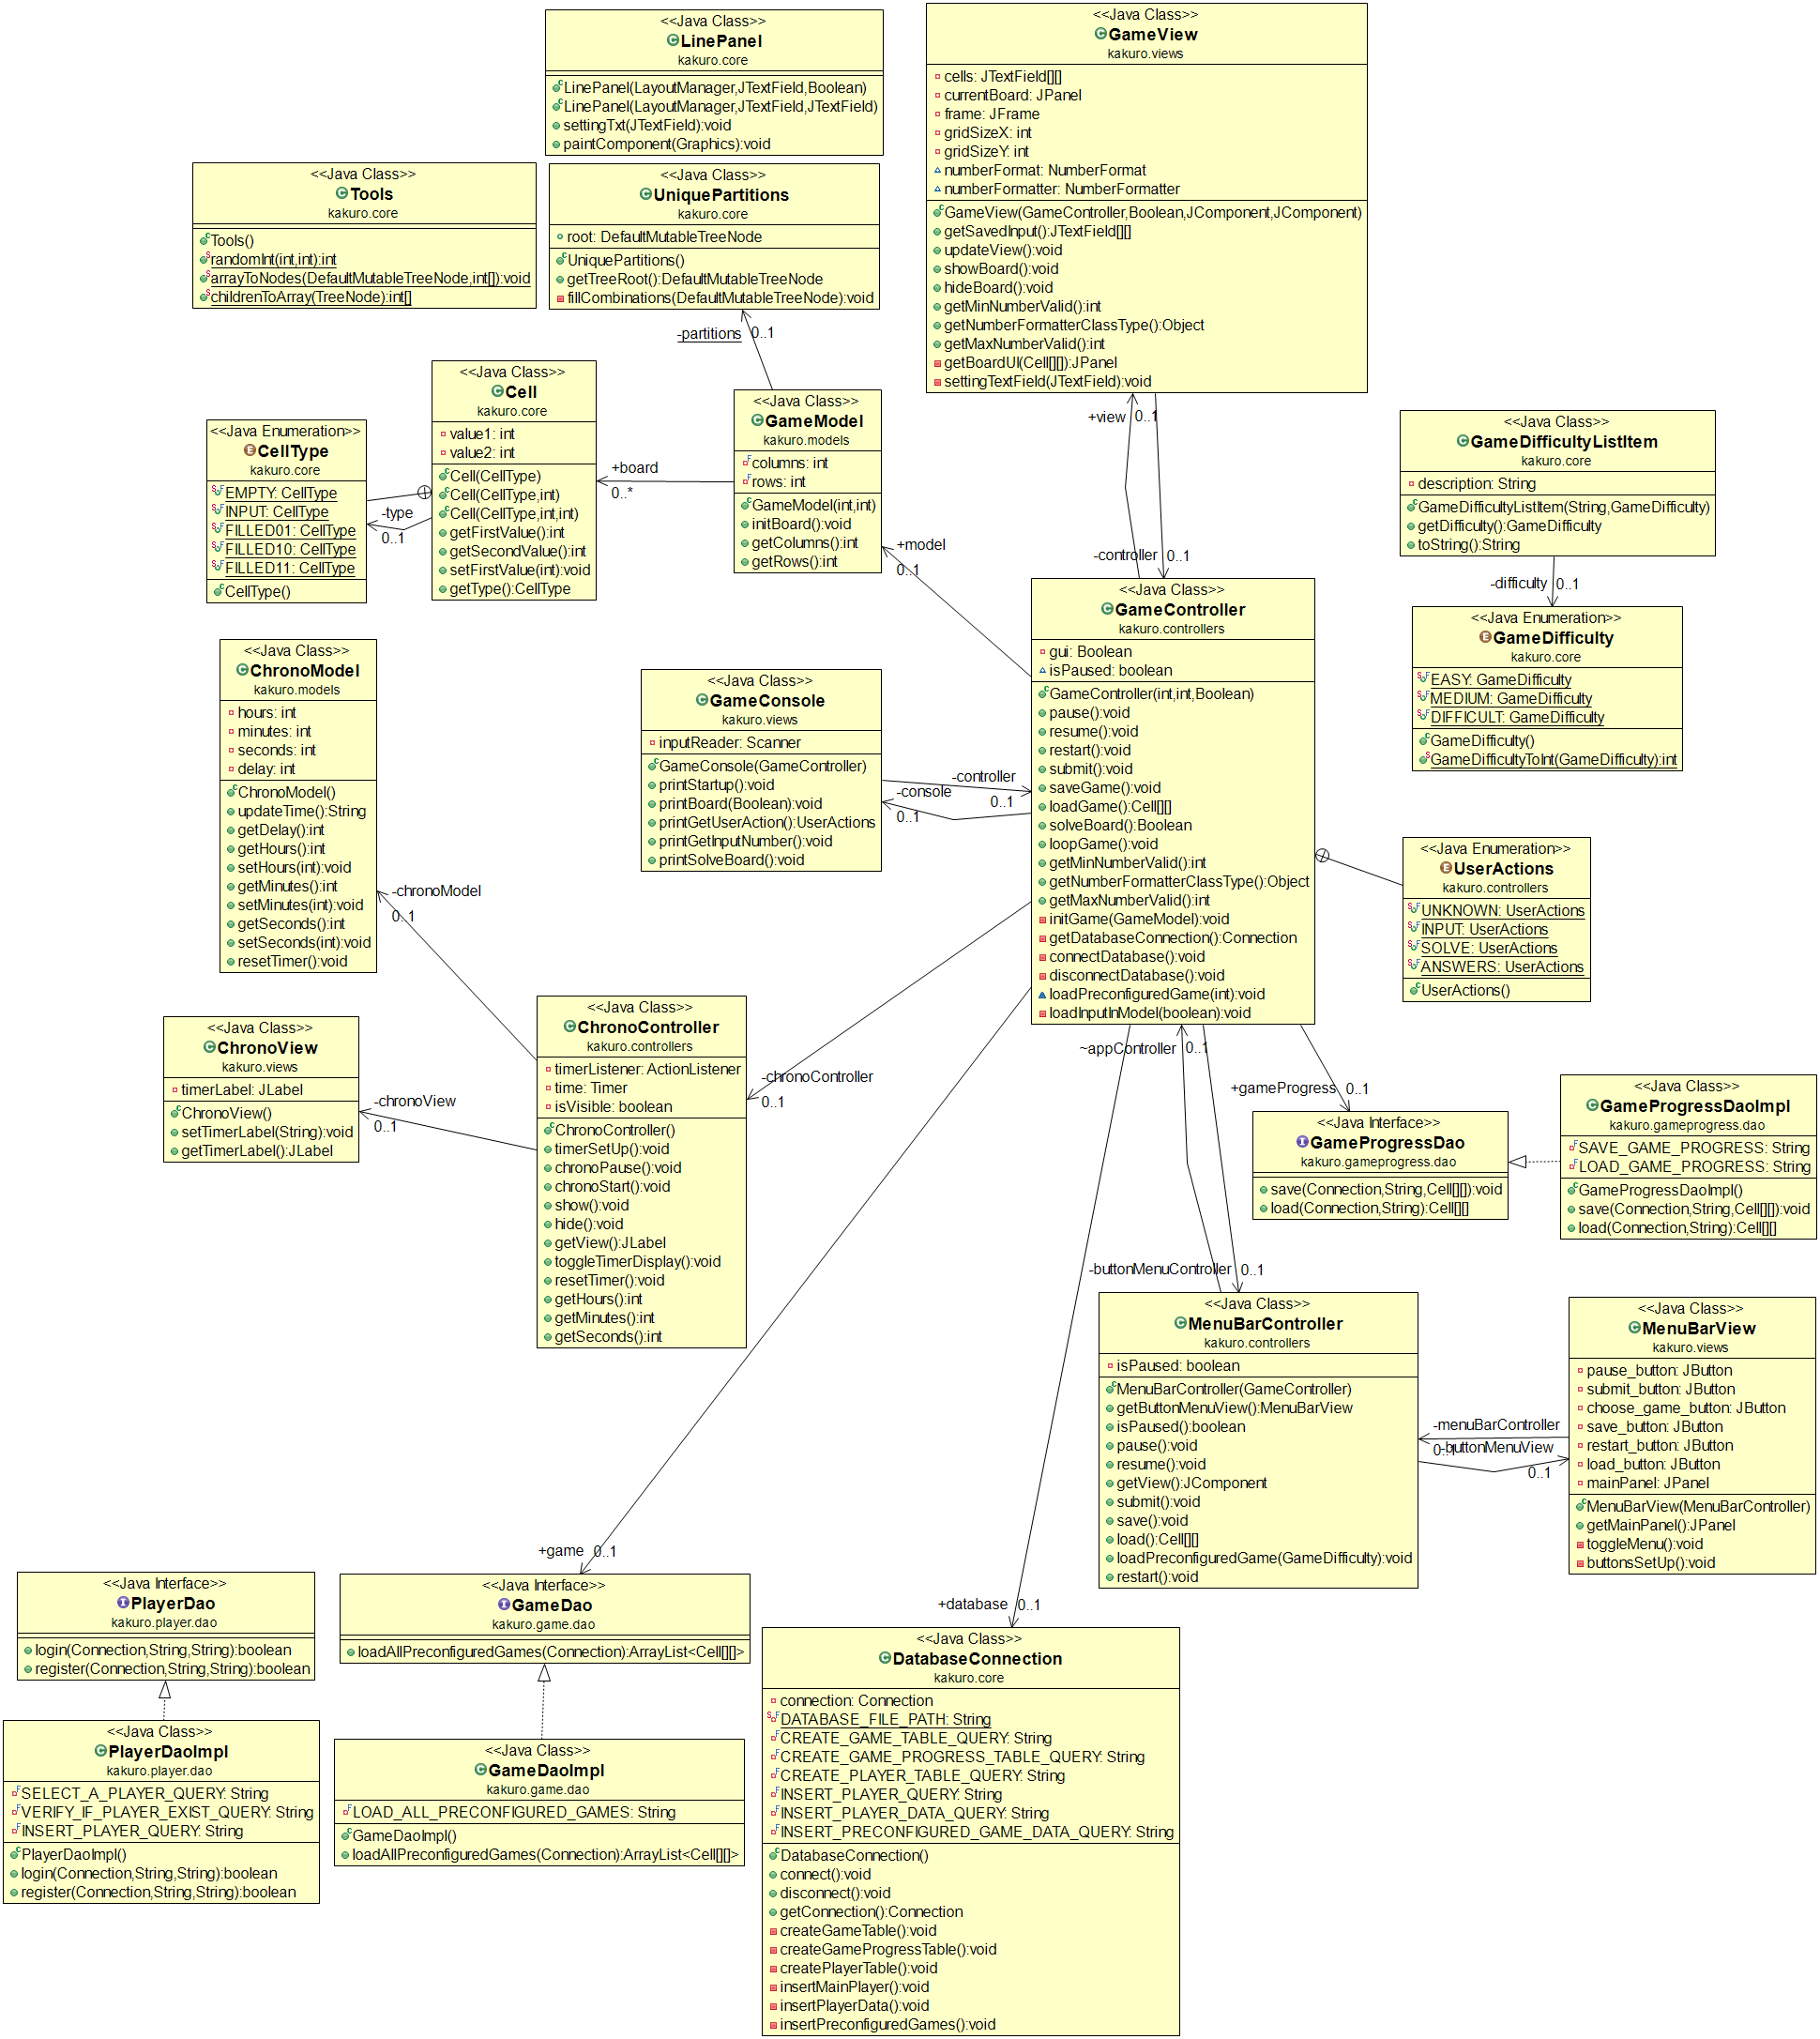
\includegraphics[width=1\textwidth]{Class_UML}
    \caption{UML of Kakuro System Class}
    \label{fig:Class_UML}
\end{figure}

\newpage

\subsection{View Module}

\subsubsection{Detailed Design Diagram}

\begin{figure}[htbp]
    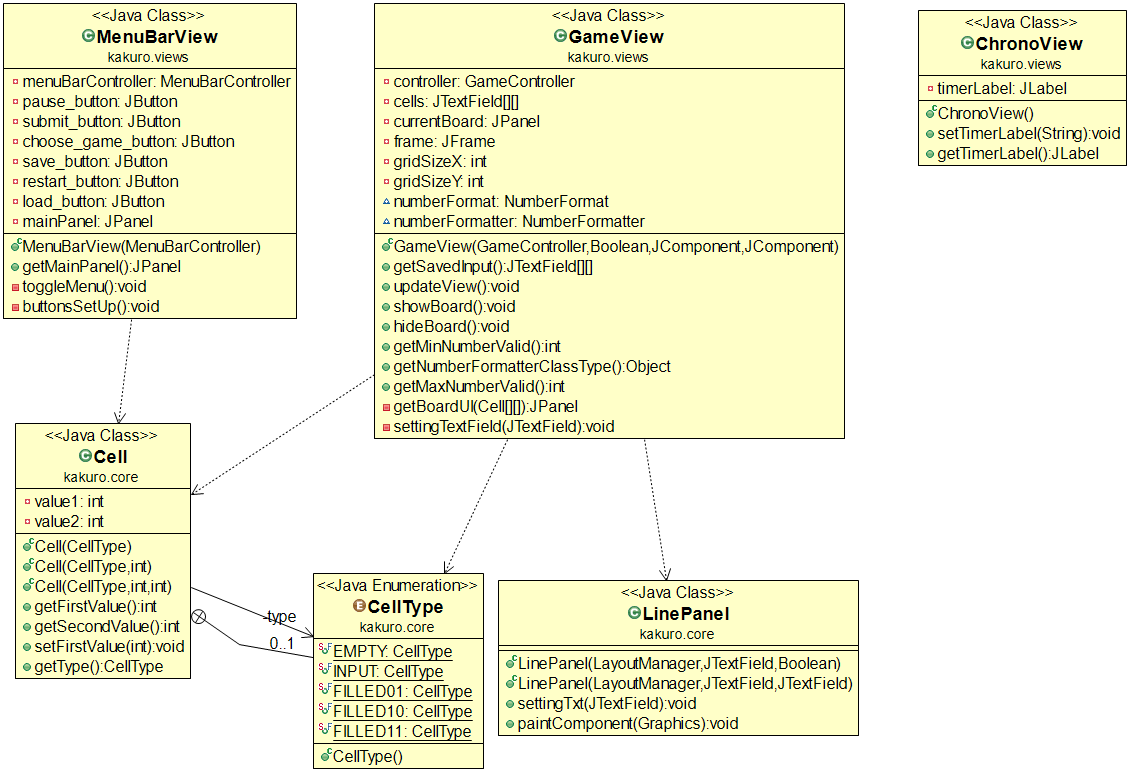
\includegraphics[width=1\textwidth]{images/View_UML.png}
    \caption{UML of View Module}
    \label{fig:View_UML}
\end{figure}

The View module can be changed easily without impacting the functionality of the Kakuro system because it takes advantage of the MVC architecture. There are three view components at the iteration 2, they are the Game view, the Menu bar view and the Chrono view, which it a timer. The View model displays the data from the Model module, and also updates itself controlled by the Controller module. The Game View module incules the LinePane and Cell class.

\newpage
\subsubsection{Units Description}

\begin{flushleft}
\begin{tabular}{| l | l | l | l |}

    \hline
    \textbf{Class Name} & \multicolumn{3}{ l |} {\textbf{GameView}} \\
    \hline
    Inherits from & \multicolumn{3}{ l |}{None} \\
    \hline
    Description & \multicolumn{3}{ l |} {Game view class which handles the Kakuro game interface} \\
    \hline
    \multirow{9}{*}{Attributes} & Visibility & Data Type & Name \\
    \cline{2-4}
     & Private & GameController & controller  \\\cline{2-4}
     & Private & JPanel & currentBoard  \\ \cline{2-4}
     & Private & JFrame & frame  \\ \cline{2-4}
     & Private & JTextField[ ][ ] & cells \\ \cline{2-4}
     & Private & int & gridSizeX  \\ \cline{2-4}
     & Private & int & gridSizeY  \\ \cline{2-4}
     & Package & NumberFormat & numberFormat \\ \cline{2-4}
     & Package & NumberFormatter & numberFormatter \\ 
    \hline
    
    \multirow{12}{*}{Methods} & Visibility & \multicolumn{2}{l |}{Method Name}  \\
    \cline{2-4}
    & Public &  \multicolumn{2}{l |}{GameView(GameController, Boolean, JComponent, JComponent)}  \\\cline{2-4}
    & Public & \multicolumn{2}{l |}{getSaveInput()} \\\cline{2-4}
    & Public & \multicolumn{2}{l |}{updateView()} \\\cline{2-4}
    & Public & \multicolumn{2}{l |}{showBoard()} \\\cline{2-4}
    & Public & \multicolumn{2}{l |}{hideBoard()} \\\cline{2-4}
    & Public & \multicolumn{2}{l |}{getNumberFormatterClassType()} \\\cline{2-4}
    & Public & \multicolumn{2}{l |}{getMinNumberValid()} \\\cline{2-4}
    & Public & \multicolumn{2}{l |}{getMaxNumberValid()} \\\cline{2-4}
    & Private & \multicolumn{2}{l |}{getBoardUI(Cell[ ][ ])} \\\cline{2-4}
    & Private & \multicolumn{2}{l |}{settingTextField(JTextField)} \\
    \hline
\end{tabular}
\end{flushleft}

\begin{flushleft}
\begin{tabular}{| l | l | l | l |}
    \hline
    \textbf{Class Name} & \multicolumn{3}{ l |} {\textbf{MenuBarView}} \\
    \hline
    Inherits from & \multicolumn{3}{ l |}{None} \\
    \hline
    Description & \multicolumn{3}{ l |} {Menu bar view class which handles buttons in the view interface} \\
    \hline
    \multirow{8}{*}{Attributes} & Visibility & Data Type & Name \\
    \cline{2-4}
    & Private & MenuBarController & menuBarController   \\\cline{2-4}
     & Private & JButton &  pause\_button  \\\cline{2-4}
      & Private & JButton &  submit\_button  \\\cline{2-4}
       & Private & JButton &  choose\_game\_button  \\\cline{2-4}
        & Private & JButton &  save\_button  \\\cline{2-4}
         & Private & JButton &  restart\_button  \\\cline{2-4}
          & Private & JButton &  load\_button  \\\cline{2-4}
     & Private & JPanel &  mainPanel  \\      
    \hline
    \multirow{5}{*}{Methods} & Visibility & \multicolumn{2}{l |}{Method Name}  \\\cline{2-4}
    & Public & \multicolumn{2}{l |}{MenuBarView(MenuBarController)} \\\cline{2-4}
    & Public & \multicolumn{2}{l |}{getMainPanel()} \\\cline{2-4}
    & Private & \multicolumn{2}{l |}{toggleMenu()} \\\cline{2-4}
     & Private & \multicolumn{2}{l |}{buttonSetUp()} \\
    \hline
\end{tabular}
\end{flushleft}

\begin{flushleft}
\begin{tabular}{| l | l | l | l |}
    \hline
    \textbf{Class Name} & \multicolumn{3}{ l |} {\textbf{ChronoView}} \\
    \hline
    Inherits from & \multicolumn{3}{ l |}{None} \\
    \hline
    Description & \multicolumn{3}{ l |} {Timer view class called Chrono, which acts as our view interface} \\
    \hline
    \multirow{2}{*}{Attributes} & Visibility & Data Type & Name \\
    \cline{2-4}
    & Private & JLabel &  timerLabel  \\
    \hline
    \multirow{4}{*}{Methods} & Visibility & \multicolumn{2}{l |}{Method Name}  \\\cline{2-4}
    & Public & \multicolumn{2}{l |}{ChronoView()} \\\cline{2-4}
    & Public & \multicolumn{2}{l |}{setTimerLabel(String)} \\\cline{2-4}
     & Public & \multicolumn{2}{l |}{getTimerLabel()} \\
    \hline
\end{tabular}
\end{flushleft}

\begin{flushleft}
\begin{tabular}{| l | l | l | l |}
    \hline
    \textbf{Class Name} & \multicolumn{3}{ l |} {\textbf{Cell}} \\
    \hline
    Inherits from & \multicolumn{3}{ l |}{None} \\
    \hline
    Description & \multicolumn{3}{ l |} {Cell class that is defines each cell in our board} \\
    \hline
    \multirow{4}{*}{Attributes} & Visibility & Data Type & Name \\
    \cline{2-4}
     & Private & int & value1 \\
     \cline{2-4}
     & Private & int & value2 \\
     \cline{2-4}
     & Package & enum & CellType  \\
    \hline
    \multirow{8}{*}{Methods} & Visibility & \multicolumn{2}{l |}{Method Name} \\
    \cline{2-4}
    & Public &   \multicolumn{2}{l |}{Cell(CellType)} \\
    \cline{2-4}
    & Public &   \multicolumn{2}{l |}{Cell(CellType, int)} \\
    \cline{2-4}
    & Public &   \multicolumn{2}{l |}{Cell(CellType, int, int)} \\
    \cline{2-4}
    & Public &   \multicolumn{2}{l |}{getFirstValue()} \\
    \cline{2-4}
    & Public &   \multicolumn{2}{l |}{getSecondValue()} \\
    \cline{2-4}
    & Public &   \multicolumn{2}{l |}{setFirstValue(int)} \\
    \cline{2-4}
    & Public &   \multicolumn{2}{l |}{getType()} \\
    \hline
\end{tabular}
\end{flushleft}

\begin{flushleft}
\begin{tabular}{| l | l | l | l |}
    \hline
    \textbf{Class Name} & \multicolumn{3}{ l |} {\textbf{LinePanel}} \\
    \hline
    Inherits from & \multicolumn{3}{ l |}{JPanel} \\
    \hline
    Description & \multicolumn{3}{ p{12cm} |} {Line panel class used to populate non-playable board cells: adds numbers and diagonal line. It is also extending JPanel to use the graphics with paintComponent() method overriding} \\
    \hline
    % \multirow{2}{*}{Attributes} & Visibility & Data Type & Name \\
    % \cline{2-4}
    % & Private &  &    \\
    % \hline
    \multirow{3}{*}{Methods} & Visibility & \multicolumn{2}{l |}{Method Name}  \\\cline{2-4}
    & Public & \multicolumn{2}{l |}{LinePanel(LayoutManager, JTextField, Boolean)} \\\cline{2-4}
    & Public & \multicolumn{2}{l |}{LinePanel(LayoutManager, JTextField, JTextField)} \\\cline{2-4}
     & Public & \multicolumn{2}{l |}{settingTxt(JTextField)} \\\cline{2-4}
     & Public & \multicolumn{2}{l |}{paintComponent(Graphics)} \\
    \hline
\end{tabular}
\end{flushleft}

\newpage

\subsection{Model Module}

\subsubsection{Detailed Design Diagram}

\begin{figure}[htbp]
    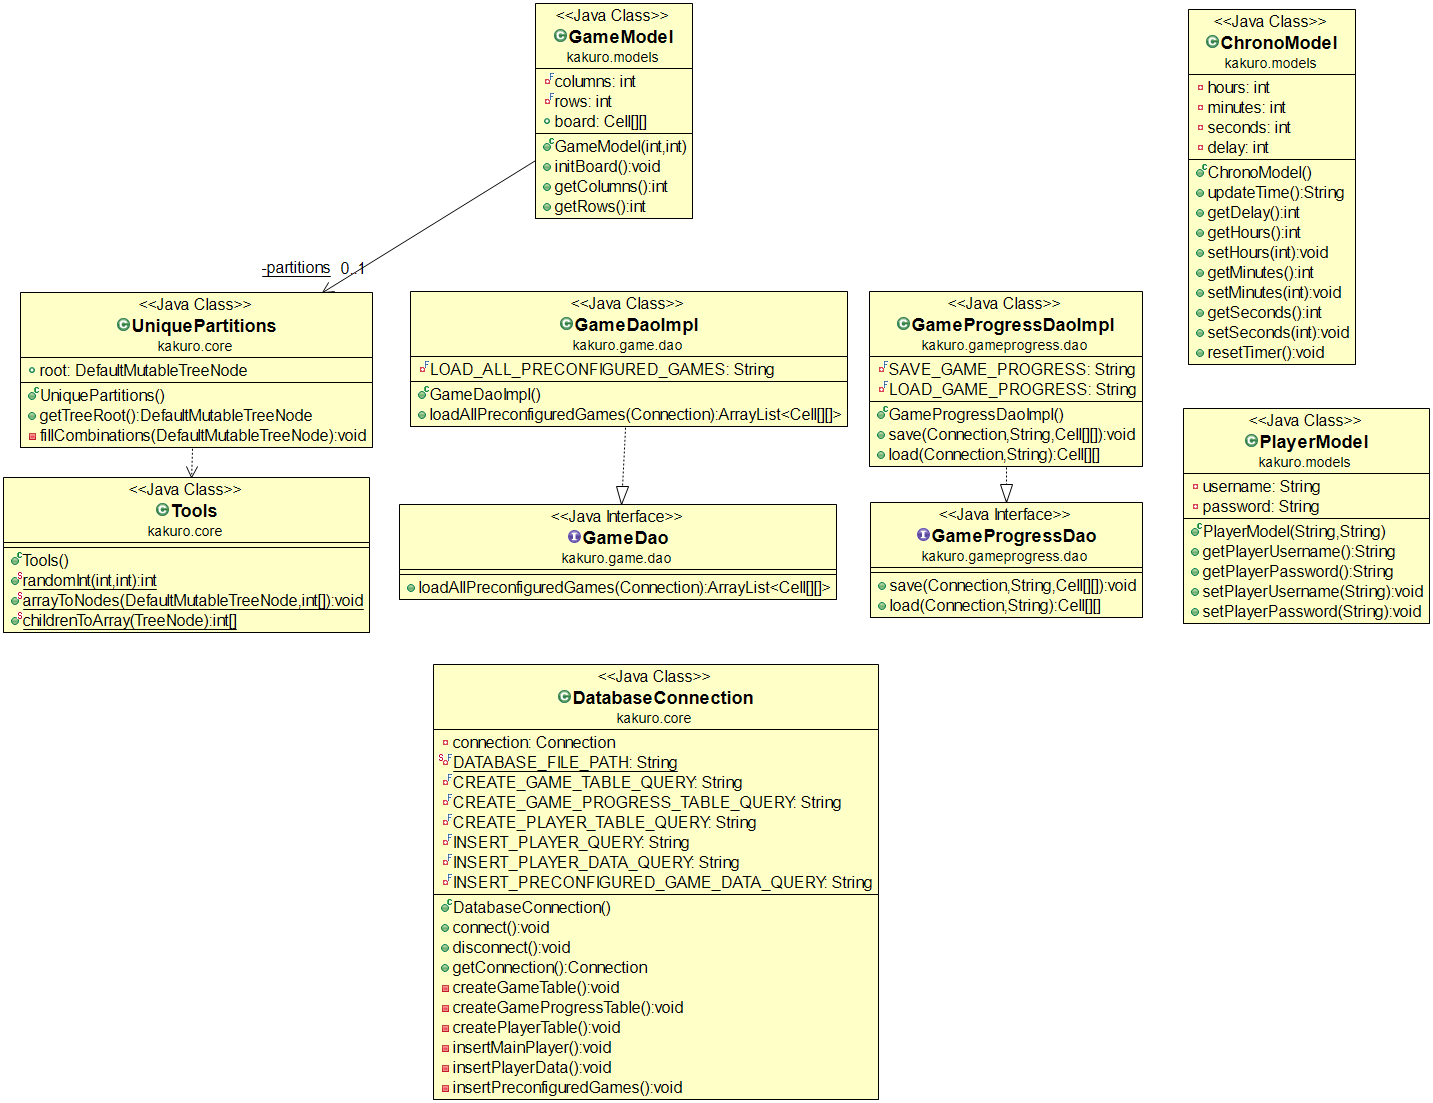
\includegraphics[width=1\textwidth]{images/Model_UML.png}
    \caption{UML of Model Module}
    \label{fig:Model_UML}
\end{figure}

The core part of the Kakuro system design is the Model module. This module is used to represent the data of the game, such as the game state, actions, timer, player data etc. Database Connection sits in this module. This module consists of three classes, GameModel, ChronoModel, and PlayerModel. Initial game board and get column and rows data are the key part of the game system. The time information are related to the game score which will be implemented in the iteration 3. The player model handles the username and password information will be used to login and register the game system, which will be implemented in iteration 3. In the iteration 2, the Game model performs the main functionality. The Model module provides the data requests from the View module, and receives and stores the data from the Controller module.The Game Model includes the UniquePartitions, Tools, DatabaseConnection, GameDaoIml and GameProgressDaoImpl class.

\newpage

\subsubsection{Units Description}

\begin{flushleft}
\begin{tabular}{| l | l | l | l |}
    \hline
    \textbf{Class Name} & \multicolumn{3}{ l |} {\textbf{GameModel}} \\
    \hline
    Inherits from & \multicolumn{3}{ l |}{None} \\
    \hline
    Description & \multicolumn{3}{ l |} {Game model class, which acts as our representation data for the object } \\
    \hline
    \multirow{5}{*}{Attributes} & Visibility & Data Type & Name \\
    \cline{2-4}
    & Private & int & columns   \\ \cline{2-4}
    & Private & int &  rows  \\ \cline{2-4}
    & Private & Cell[ ][ ] &  board  \\ \cline{2-4}
    & Private & UniquePartitions &  partitions  \\ 
    \hline
    \multirow{5}{*}{Methods} & Visibility & \multicolumn{2}{l |}{Method Name}  \\\cline{2-4}
    & Public & \multicolumn{2}{l |}{GameModel(int, int)} \\\cline{2-4}
     & Public & \multicolumn{2}{l |}{initBoard()} \\\cline{2-4}
      & Public & \multicolumn{2}{l |}{getColumns()} \\\cline{2-4}
     & Public & \multicolumn{2}{l |}{getRows()} \\
    \hline
\end{tabular}
\end{flushleft}

\begin{flushleft}
\begin{tabular}{| l | l | l | l |}
    \hline
    \textbf{Class Name} & \multicolumn{3}{ l |} {\textbf{PlayerModel}} \\
    \hline
    Inherits from & \multicolumn{3}{ l |}{None} \\
    \hline
    Description & \multicolumn{3}{ l |} {Player model class, which acts as our representation data for the object} \\
    \hline
    \multirow{3}{*}{Attributes} & Visibility & Data Type & Name \\
    \cline{2-4}
    & Private & String &  username  \\ \cline{2-4}
    & Private & String & password   \\
    \hline
    \multirow{6}{*}{Methods} & Visibility & \multicolumn{2}{l |}{Method Name}  \\\cline{2-4}
    & Public & \multicolumn{2}{l |}{PlayerModel(String, String)} \\\cline{2-4}
     & Public & \multicolumn{2}{l |}{getPlayerUsername()} \\\cline{2-4}
      & Public & \multicolumn{2}{l |}{getPlayerPassword()} \\\cline{2-4}
       & Public & \multicolumn{2}{l |}{setPlayerUsername(String)} \\\cline{2-4}
     & Public & \multicolumn{2}{l |}{setPlayerPassword(String)} \\
    \hline
\end{tabular}
\end{flushleft}

\begin{flushleft}
\begin{tabular}{| l | l | l | l |}
    \hline
    \textbf{Class Name} & \multicolumn{3}{ l |} {\textbf{ChronoModel}} \\
    \hline
    Inherits from & \multicolumn{3}{ l |}{None} \\
    \hline
    Description & \multicolumn{3}{ l |} {Timer model acts as our representation data for the object} \\
    \hline
    \multirow{5}{*}{Attributes} & Visibility & Data Type & Name \\
    \cline{2-4}
    & Private & int & hours   \\\cline{2-4}
    & Private & int & minutes   \\\cline{2-4}
    & Private & int & seconds   \\\cline{2-4}
    & Private & int & delay   \\
    \hline
    \multirow{11}{*}{Methods} & Visibility & \multicolumn{2}{l |}{Method Name}  \\\cline{2-4}
    & Public & \multicolumn{2}{l |}{ChronoModel()} \\\cline{2-4}
    & Public & \multicolumn{2}{l |}{updateTime()} \\\cline{2-4}
    & Public & \multicolumn{2}{l |}{getDelay()} \\\cline{2-4}
    & Public & \multicolumn{2}{l |}{getHours()} \\\cline{2-4}
    & Public & \multicolumn{2}{l |}{setHour(int)} \\\cline{2-4}
    & Public & \multicolumn{2}{l |}{getMinutes()} \\\cline{2-4}
    & Public & \multicolumn{2}{l |}{setMinutes(int)} \\\cline{2-4}
    & Public & \multicolumn{2}{l |}{getSecounds()} \\\cline{2-4}
    & Public & \multicolumn{2}{l |}{setSeconds(int)} \\\cline{2-4}
     & Public & \multicolumn{2}{l |}{resetTimer()} \\
    \hline
\end{tabular}
\end{flushleft}

\begin{flushleft}
\begin{tabular}{| l | l | l | l |}
    \hline
    \textbf{Class Name} & \multicolumn{3}{ l |} {\textbf{UniquePartitions}} \\
    \hline
    Inherits from & \multicolumn{3}{ l |}{None} \\
    \hline
    Description & \multicolumn{3}{ l |} {Lists all possible answers in a Tree ADT} \\
    \hline
    \multirow{2}{*}{Attributes} & Visibility & Data Type & Name \\
    \cline{2-4}
     & Private & DefaultMutableTreeNode & root  \\
    \hline
    \multirow{4}{*}{Methods} & Visibility & \multicolumn{2}{l |}{Method Name} \\
    \cline{2-4}
    & Public &   \multicolumn{2}{l |}{UniquePartitions()} \\
    \cline{2-4}
    & Public &   \multicolumn{2}{l |}{getTreeRoot()} \\
    \cline{2-4}
    & Public &   \multicolumn{2}{l |}{fillCombinations(DefaultMutableTreeNode)}\\
    \hline
\end{tabular}
\end{flushleft}

\begin{flushleft}
\begin{tabular}{| l | l | l | l | l |}
    \hline
    \textbf{Class Name} & \multicolumn{3}{ l |} {\textbf{Tools}} \\
    \hline
    Inherits from & \multicolumn{3}{ l |}{None} \\
    \hline
    Description & \multicolumn{3}{ l |} {Tools for general utilities} \\
    \hline
    % \multirow{2}{*}{Attributes} & Visibility & Data Type & Name & Description \\
    % \cline{2-5}
    %  & Private &  &  &  \\
    % \hline
    \multirow{5}{*}{Methods} & Visibility &   \multicolumn{2}{l |}{Method Name} \\
    \cline{2-4}
    & Public &   \multicolumn{2}{l |}{Tools()} \\
    \cline{2-4}
    & Public &   \multicolumn{2}{l |}{randomInt(int, int)} \\
    \cline{2-4}
    & Public &   \multicolumn{2}{l |}{arrayToNodes(DefaultMutableTreeNode, int[ ])} \\
    \cline{2-4}
    & Public &   \multicolumn{2}{l |}{childrenToArray(TreeNode)} \\
    \hline
\end{tabular}
\end{flushleft}

\begin{flushleft}
\begin{tabular}{| l | l | l | l |}
    \hline
    \textbf{Class Name} & \multicolumn{3}{ l |} {\textbf{GameDaoImpl}} \\
    \hline
    Implements from & \multicolumn{3}{ l |}{GameDao} \\
    \hline
    Description & \multicolumn{3}{ p{12cm} |} {Game implementation class that implements the abstract class for operations in the database} \\
    \hline
    \multirow{2}{*}{Attributes} & Visibility & Data Type & Name  \\
    \cline{2-4}
     & Private & String  & LOAD\_ALL\_PRECONFIGURED\_GAMES \\
    \hline
    \multirow{3}{*}{Methods} & Visibility & \multicolumn{2}{ l |}{Method Name}  \\
    \cline{2-4}
    & Public & \multicolumn{2}{ l |}{GameDaoImpl()}  \\
    \cline{2-4}
    & Public & \multicolumn{2}{ l |}{loadAllPreconfiguredGames(Connection)}  \\
    \hline
\end{tabular}
\end{flushleft}

\begin{flushleft}
\begin{tabular}{| l | l | l | l | l |}
    \hline
    \textbf{Class Name} & \multicolumn{3}{ l |} {\textbf{GameProgressDaoImpl}} \\
    \hline
    Implements from & \multicolumn{3}{ l |}{GameProgressDao} \\
    \hline
    Description & \multicolumn{3}{ p{12cm} |} {Game Progress implementation class that implements the abstract class for operations in the database} \\
    \hline
    \multirow{3}{*}{Attributes} & Visibility & Data Type & Name \\
    \cline{2-4}
     & Private & String & SAVE\_GAME\_PROGRESS  \\
    \cline{2-4}
     & Private & String &  LOAD\_GAME\_PROGRESS  \\
    \hline
    \multirow{4}{*}{Methods} & Visibility &  \multicolumn{2}{ l |}{Method Name}  \\
    \cline{2-4}
    & Public & \multicolumn{2}{ l |}{GameProgressDaoImpl()} \\
    \cline{2-4}
    & Public & \multicolumn{2}{ l |}{save(Connection, String, Cell[ ][ ])}  \\
    \cline{2-4}
    & Public & \multicolumn{2}{ l |}{load(Connection, String)}  \\
    \hline
\end{tabular}
\end{flushleft}

\begin{flushleft}
\begin{tabular}{| l | l | l | l |}
    \hline
    \textbf{Class Name} & \multicolumn{3}{ l |} {\textbf{DatabaseConnection}} \\
    \hline
    Inherits from & \multicolumn{3}{ l |}{None} \\
    \hline
    Description & \multicolumn{3}{ p{15cm} |} {Database connection class to create the connection to our database, which creates the database, tables and inserts preloaded data if they do not exist} \\
    \hline
    \multirow{9}{*}{Attributes} & Visibility & Data Type & Name \\
    \cline{2-4}
    & Private & Connection &  connection  \\\cline{2-4}
    & Private & String & DATABASE\_FILE\_PATH   \\\cline{2-4}
    & Private & String & CREATE\_GAME\_PROGRESS\_TABLE\_QUERY   \\\cline{2-4}
    & Private & String & CREATE\_PLAYER\_TABLE\_QUERY   \\\cline{2-4}
    & Private & String & INSERT\_PLAYER\_QUERY   \\\cline{2-4}
    & Private & String & INSERT\_PLAYER\_DATA\_QUERY   \\\cline{2-4}
    & Private & String & INSERT\_PRECONFIGURED\_GAME\_DATA\_QUERY   \\
    \hline
    \multirow{3}{*}{Methods} & Visibility & \multicolumn{2}{l |}{Method Name}  \\\cline{2-4}
    & Public & \multicolumn{2}{l |}{DatabaseConnection()} \\\cline{2-4}
    & Public & \multicolumn{2}{l |}{connect()} \\\cline{2-4}
    & Public & \multicolumn{2}{l |}{disconnect()} \\\cline{2-4}
    & Public & \multicolumn{2}{l |}{getConnection()} \\\cline{2-4}
     & Private & \multicolumn{2}{l |}{createGameTable()} \\\cline{2-4}
     & Private & \multicolumn{2}{l |}{createGameProgressTable()} \\\cline{2-4}
     & Private & \multicolumn{2}{l |}{createPlayerTable()} \\\cline{2-4}
     & Private & \multicolumn{2}{l |}{insertMainPlayer()} \\\cline{2-4}
     & Private & \multicolumn{2}{l |}{insertPlayerData()} \\\cline{2-4}
     & Private & \multicolumn{2}{l |}{insertPreconfiuredGames()} \\
    \hline
\end{tabular}
\end{flushleft}

\newpage

\subsection{Controller Module}

\subsubsection{Detailed Design Diagram}


\begin{figure}[htbp]
    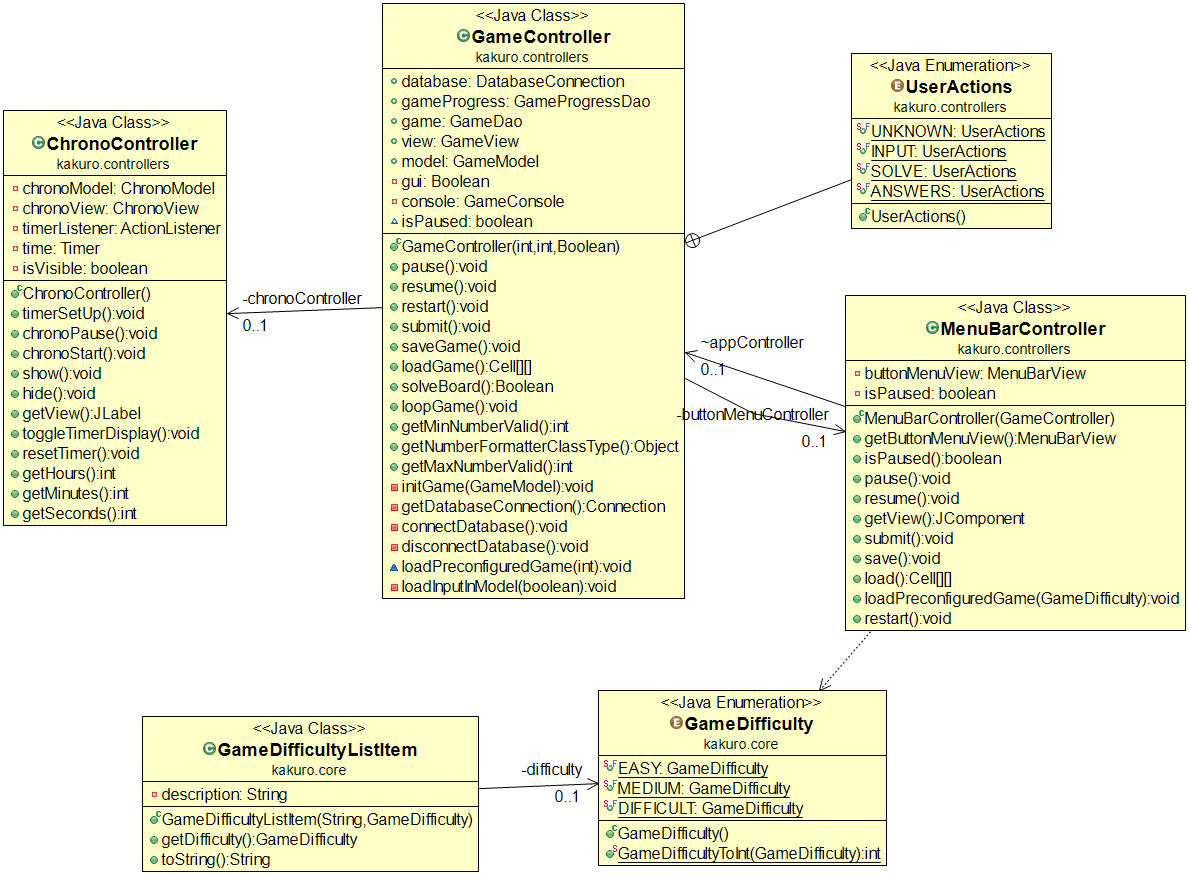
\includegraphics[width=1\textwidth]{images/Controller_UML.png}
    \caption{UML of Controller Module}
    \label{fig:Controller_UML}
\end{figure}

The Controller module orchestrates the Model module and View module of the Karuro system. The Game Controller accepts input from the player and the button click events, and it also validates the input checking and notifies the user. The Controller module handles the data flows between the Model module and the View module. It handles connection and disconnection to the database. It also save game, load game, pause game, resume game, and restart game through the Menu bar controller. The Chrono controller is a timer controller, and it handles all time related functionality. The Game Controller module includes the MenuBarController, ChronoController and GameDifficultyListItem class.

\subsubsection{Units Description}

\begin{flushleft}
\begin{tabular}{| l | l | l | l |}
    \hline
    \textbf{Class Name} & \multicolumn{3}{ l |} {\textbf{GameController}} \\
    \hline
    Inherits from & \multicolumn{3}{ l |}{None} \\
    \hline
    Description & \multicolumn{3}{ l |} {Basically orchestrates the model and view of the game} \\
    \hline
    \multirow{10}{*}{Attributes} & Visibility & Data Type & Name \\
    \cline{2-4}
    & Public & DatabaseConnection & database   \\\cline{2-4}
    & Public & GameProgressDao & gameProgress   \\\cline{2-4}
    & Public & GameDao & game   \\\cline{2-4}
    & Public & GameView &  view  \\\cline{2-4}
    & Public & GameModel & model  \\\cline{2-4}
    & Public & enum & UserActions   \\\cline{2-4}
    & Private & Boolean &  gui  \\\cline{2-4}
    & Private & GameConsole & console   \\\cline{2-4}
    & Package & boolean & isPaused   \\
    \hline
    \multirow{20}{*}{Methods} & Visibility & \multicolumn{2}{l |}{Method Name}  \\\cline{2-4}
    & Public & \multicolumn{2}{l |}{GameController(int, int, Boolean)} \\\cline{2-4}
    & Public & \multicolumn{2}{l |}{UserActions()} \\\cline{2-4}
    & Public & \multicolumn{2}{l |}{pause()} \\\cline{2-4}
    & Public & \multicolumn{2}{l |}{resume()} \\\cline{2-4}
    & Public & \multicolumn{2}{l |}{restart()} \\\cline{2-4}
    & Public & \multicolumn{2}{l |}{submit()} \\\cline{2-4}
    & Public & \multicolumn{2}{l |}{saveGame()} \\\cline{2-4}
    & Public & \multicolumn{2}{l |}{loadGame()} \\\cline{2-4}
    & Public & \multicolumn{2}{l |}{solveBoard()} \\\cline{2-4}
    & Public & \multicolumn{2}{l |}{loopGame()} \\\cline{2-4}
    & Public & \multicolumn{2}{l |}{getMinNumberValid()} \\\cline{2-4}
    & Public & \multicolumn{2}{l |}{getNumberFormatterClassType()} \\\cline{2-4}
    & Public & \multicolumn{2}{l |}{getMaxNumberValid()} \\\cline{2-4}
    & Public & \multicolumn{2}{l |}{initGame(GameModel)} \\\cline{2-4}
    & Private & \multicolumn{2}{l |}{getDatabaseConnection()} \\\cline{2-4}
    & Private & \multicolumn{2}{l |}{connectDatabase()} \\\cline{2-4}
    & Private & \multicolumn{2}{l |}{disconnectDatabase()} \\\cline{2-4}
    & Private & \multicolumn{2}{l |}{loadInputInModel(boolean)} \\\cline{2-4}
   & Package & \multicolumn{2}{l |}{loadPreconfiguredGame(int)} \\
    \hline
\end{tabular}
\end{flushleft}

\begin{flushleft}
\begin{tabular}{| l | l | l | l |}
    \hline
    \textbf{Class Name} & \multicolumn{3}{ l |} {\textbf{ChronoController}} \\
    \hline
    Inherits from & \multicolumn{3}{ l |}{None} \\
    \hline
    Description & \multicolumn{3}{ l |} {Timer controller acts as an orchestrator between the model and the view} \\
    \hline
    \multirow{6}{*}{Attributes} & Visibility & Data Type & Name \\
    \cline{2-4}
    & Private & ChronoModel & chronoModel   \\\cline{2-4}
     & Private & ChronoView & chronoView   \\\cline{2-4}
      & Private & ActionListener & timerListener   \\\cline{2-4}
       & Private & Timer & time   \\\cline{2-4}
    & Private & boolean & isPaused   \\
    \hline
    \multirow{13}{*}{Methods} & Visibility & \multicolumn{2}{l |}{Method Name}  \\\cline{2-4}
    & Public & \multicolumn{2}{l |}{ChronoController()} \\\cline{2-4}
    & Public & \multicolumn{2}{l |}{timerSetUp()} \\\cline{2-4}
    & Public & \multicolumn{2}{l |}{chronoPause()} \\\cline{2-4}
    & Public & \multicolumn{2}{l |}{chronoStart()} \\\cline{2-4}
    & Public & \multicolumn{2}{l |}{show()} \\\cline{2-4}
    & Public & \multicolumn{2}{l |}{hide()} \\\cline{2-4}
    & Public & \multicolumn{2}{l |}{getView()} \\\cline{2-4}
    & Public & \multicolumn{2}{l |}{toggleTimerDisplay()} \\\cline{2-4}
    & Public & \multicolumn{2}{l |}{resetTimer()} \\\cline{2-4}
    & Public & \multicolumn{2}{l |}{getHours()} \\\cline{2-4}
    & Public & \multicolumn{2}{l |}{getMinutes()} \\\cline{2-4}
     & Public & \multicolumn{2}{l |}{getSeconds()} \\
    \hline
\end{tabular}
\end{flushleft}

\begin{flushleft}
\begin{tabular}{| l | l | l | l |}
    \hline
    \textbf{Class Name} & \multicolumn{3}{ l |} {\textbf{MenuBarController}} \\
    \hline
    Inherits from & \multicolumn{3}{ l |}{None} \\
    \hline
    Description & \multicolumn{3}{ l |} {Handles the buttons in our game application} \\
    \hline
    \multirow{3}{*}{Attributes} & Visibility & Data Type & Name \\
    \cline{2-4}
    & Private & MenuBarView & buttonMenuView   \\\cline{2-4}
    & Private & boolean & isPaused   \\
    \hline
    \multirow{12}{*}{Methods} & Visibility & \multicolumn{2}{l |}{Method Name}  \\\cline{2-4}
    & Public & \multicolumn{2}{l |}{MenuBarController(GameController)} \\\cline{2-4}
    & Public & \multicolumn{2}{l |}{getButtonMenuView()} \\\cline{2-4}
    & Public & \multicolumn{2}{l |}{isPaused()} \\\cline{2-4}
    & Public & \multicolumn{2}{l |}{pause()} \\\cline{2-4}
    & Public & \multicolumn{2}{l |}{resume()} \\\cline{2-4}
    & Public & \multicolumn{2}{l |}{getView()} \\\cline{2-4}
    & Public & \multicolumn{2}{l |}{submit()} \\\cline{2-4}
    & Public & \multicolumn{2}{l |}{save()} \\\cline{2-4}
    & Public & \multicolumn{2}{l |}{load()} \\\cline{2-4}
    & Public & \multicolumn{2}{l |}{loadPreConfiguredGame(GameDifficulty)} \\\cline{2-4}
     & Public & \multicolumn{2}{l |}{restart()} \\
    \hline
\end{tabular}
\end{flushleft}

\begin{flushleft}
\begin{tabular}{| l | l | l | l |}
    \hline
    \textbf{Class Name} & \multicolumn{3}{ l |} {\textbf{GameDifficulty}} \\
    \hline
    Inherits from & \multicolumn{3}{ l |}{None} \\
    \hline
    Description & \multicolumn{3}{ l |} {An enumerator for different levels of game difficulties} \\
    \hline
    % \multirow{2}{*}{Attributes} & Visibility & Data Type & Name \\
    % \cline{2-4}
    % & Private &  &    \\
    % \hline
    \multirow{3}{*}{Methods} & Visibility & \multicolumn{2}{l |}{Method Name}  \\\cline{2-4}
    & Public & \multicolumn{2}{l |}{GameDifficulty()} \\\cline{2-4}
     & Public & \multicolumn{2}{l |}{GameDifficultyToInt(GameDifficulty)} \\
    \hline
\end{tabular}
\end{flushleft}

\begin{flushleft}
\begin{tabular}{| l | l | l | l |}
    \hline
    \textbf{Class Name} & \multicolumn{3}{ l |} {\textbf{GameDifficultyListItem}} \\
    \hline
    Inherits from & \multicolumn{3}{ l |}{None} \\
    \hline
    Description & \multicolumn{3}{ l |} {The game difficulty found in the dropdown menu when pre-loading a game} \\
    \hline
    \multirow{3}{*}{Attributes} & Visibility & Data Type & Name \\
    \cline{2-4}
    & Private & String &  description  \\ \cline{2-4}
    & Private & GameDifficulty &  difficulty  \\
    \hline
    \multirow{3}{*}{Methods} & Visibility & \multicolumn{2}{l |}{Method Name}  \\\cline{2-4}
    & Public & \multicolumn{2}{l |}{GameDifficultyListItem(String, GameDifficulty)} \\\cline{2-4}
    & Public & \multicolumn{2}{l |}{getDifficulty()} \\\cline{2-4}
     & Public & \multicolumn{2}{l |}{toString()} \\
    \hline
\end{tabular}
\end{flushleft}

\newpage

\section{Dynamic Design Scenarios}
The following are the descriptions of the execution scenarios of the game initialization, the process of saving a game and the process of loading a game. These systems are involved in the subsystem of the puzzle mechanics.

\subsection{Initialize Game (UI only)}

In iteration 2, we do not yet have a "start game" button implemented in the UI of the game. Therefore, a use case for the current iteration is clicking of the run main button of Eclipse, which initializes the game. We also have a version of the game that can be played on the console, but for this sequence diagram, only the methods implicated in the UI of the game are involved. 
\begin{figure}[htbp]
    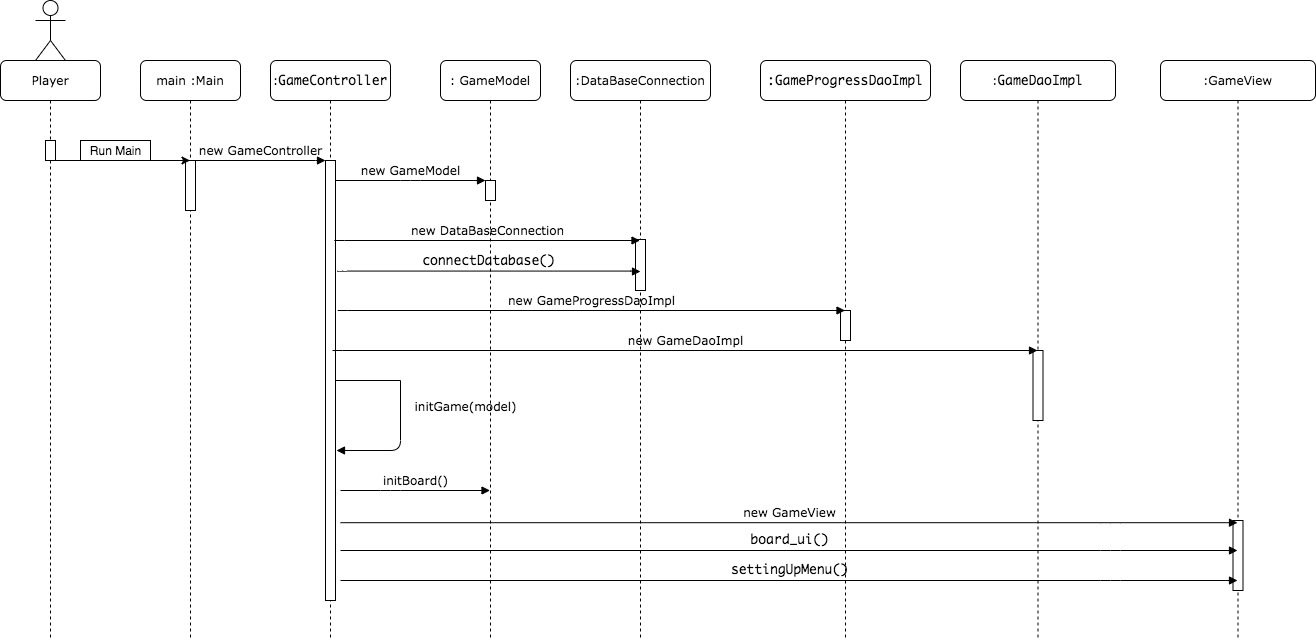
\includegraphics[width=1\textwidth]{initGame}
    \caption{Sequence diagram to initialize a game}
    \label{fig:sequenceDiagram}
\end{figure}

\newpage

\subsection{Save Game}
A crucial use case for iteration 2 that has been implemented is to save the game. Once the player has initialized the game by clicking run main, they can next choose a game level and input numbers from 1 to 9 in the board cells. If they haven't finished the game and wish to continue at a later date, this is the use case that represents this eventuality of user interaction.
\begin{figure}[htbp]
    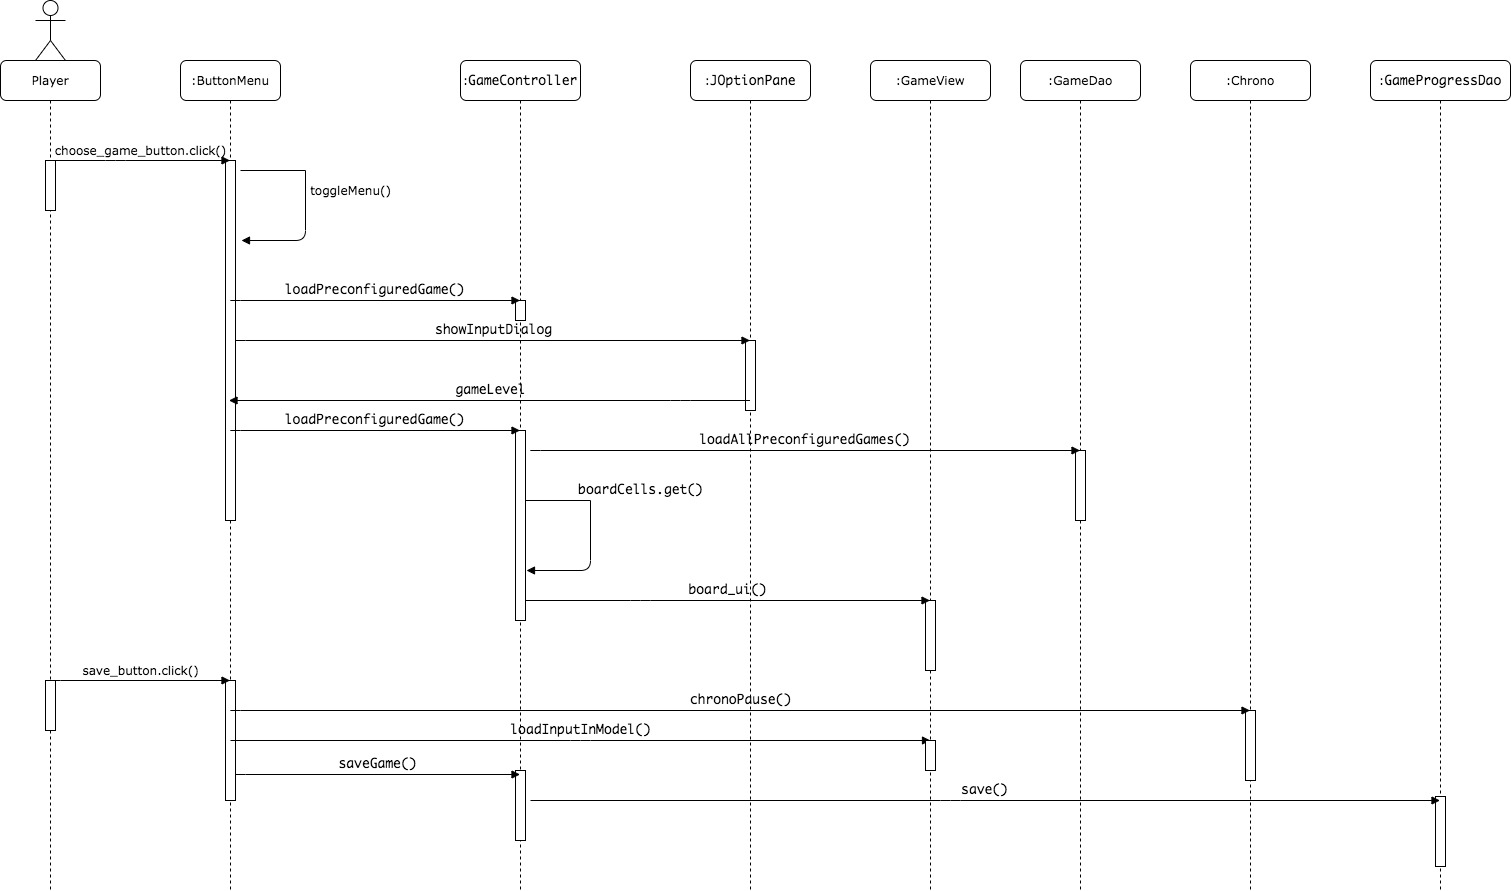
\includegraphics[width=1\textwidth]{saveGame}
    \caption{Sequence diagram to save a game}
    \label{fig:sequenceDiagram}
\end{figure}

\newpage

\subsection{Load Game}
A use case that goes hand in hand with saving the game is loading the game. Once a player has saved an in progess game, they can come back to it by loading the game they were previously playing. This is done by clicking the UI button "Load Game". This action populates the board of the game with saved inputs and the saved time value of the timer.
\begin{figure}[htbp]
    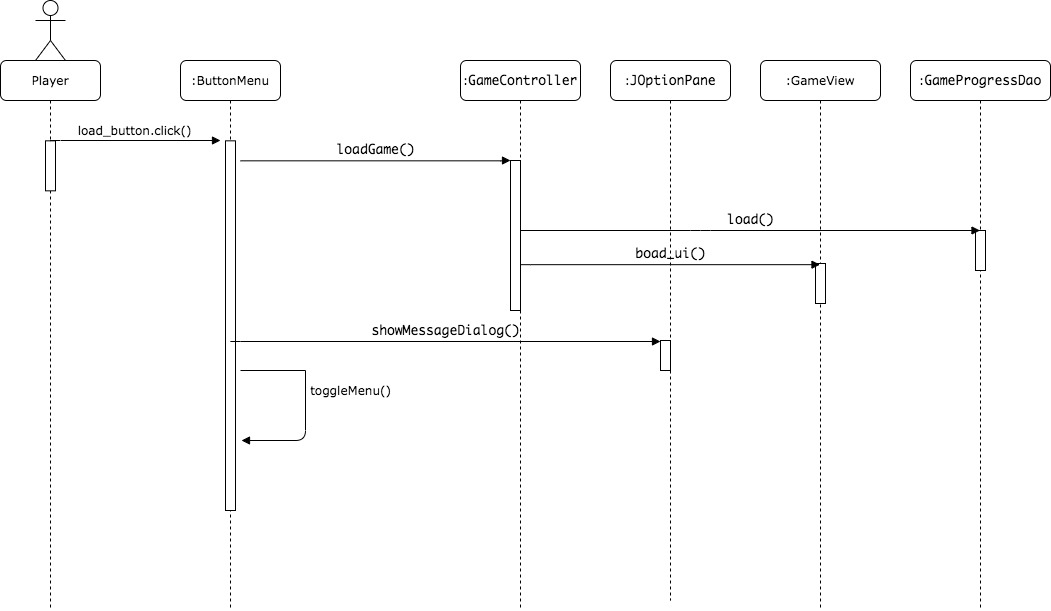
\includegraphics[width=1\textwidth]{loadGame}
    \caption{Sequence diagram to load a game}
    \label{fig:sequenceDiagram}
\end{figure}
\end{document}
